\documentclass[french,12pt]{exam}

%\printanswers

\usepackage{../../latex/macro_mealor}
\usepackage[utf8]{inputenc}
\usepackage[T1]{fontenc} % accents codés dans la fonte
%\usepackage{layout}
\usepackage{a4wide}
%\usepackage[french]{babel}
\usepackage{hyperref}

\usepackage{graphicx}
\usepackage{caption}

\usepackage{newpxtext,newpxmath}
\usepackage{siunitx}

%\setlength{\hoffset}{0pt}
%\setlength{\oddsidemargin}{-1cm}   % Marge gauche sur pages impaires
%\setlength{\evensidemargin}{-1cm}   % Marge gauche sur pages paires
%\setlength{\marginparwidth}{0cm}   % Largeur de note dans la marge
%\setlength{\textwidth}{16cm}   % Largeur de la zone de texte (17cm)
\setlength{\voffset}{0pt}   % Bon pour DOS
\setlength{\marginparsep}{0pt}   % Séparation de la marge
\setlength{\topmargin}{0cm}   % Pas de marge en haut
\setlength{\headheight}{0cm}   % Haut de page
\setlength{\headsep}{0cm}   % Entre le haut de page et le texte
%\setlength{\footskip}{1cm}   % Bas de page + séparation
%\setlength{\textheight}{25.5cm}   % Hauteur de la zone de texte (25cm)

\usepackage{indentfirst}


\newcommand{\classurl}{\url{1}}
% #1 numéro de la feuille
% #2 titre de la feuille
\newcommand{\titre}[3] {%\textit{
  \begin{center}\textbf{\textsc{MEALOR II}}\\ \textit{Mécanique de l'endommagement et approche locale de la rupture}%\let\thefootnote\relax\footnotetext{\classurl} 
  \end{center}
 
  \noindent TD n\textdegree #1 \hfill  August 2023\\[-0.3cm]
  \rule{\linewidth}{.3mm}
  \vspace*{0.5pt}
  \begin{center}
    {
      \Large \bfseries { #2}
    }\\
    \vspace*{0.5cm}
	\large #3
    \vspace*{0.5cm}
  \end{center}
}

\usepackage{xcolor}
\definecolor{Blue}{RGB}{0,68,170}
\SolutionEmphasis{\normalfont\color{Blue}}
\DeclareCaptionFont{blue}{\color{Blue}}

\newenvironment{objectifs}
    {\itshape\underline{Objectifs:}\begin{itemize}
    }
    { \itshape
    \end{itemize}
    }
    
\newcounter{Rfig}
\newenvironment{R_figure}
   {\begin{minipage}{\linewidth}\begin{center}\vspace{0.5mm}\stepcounter{Rfig}\addtocounter{figure}{-1}\renewcommand\thefigure{R-\arabic{Rfig}}
   \captionsetup{font=blue}}
   {\end{center}\vspace{0.5mm}\end{minipage}}
   
    
\newcounter{Rtab}
\newenvironment{R_table}
   {\begin{minipage}{\linewidth}\begin{center}\vspace{0.5mm}\stepcounter{Rtab}\addtocounter{table}{-1}\renewcommand\thetable{R-\arabic{Rtab}}
   \captionsetup{font=blue}
}
   {\end{center}\vspace{0.5mm}\end{minipage}}
   
      
\renewcommand{\sessionType}{TP}

\definecolor{My_green}{RGB}{0,154,0}
\definecolor{mygray}{rgb}{0.9,0.9,0.9}
\usepackage[procnames]{listings}
\lstset{language=python,
	backgroundcolor=\color{mygray},   % choose the background color; you must add \usepackage{color} or \usepackage{xcolor}; should come as last argument
  basicstyle=\footnotesize,        % the size of the fonts that are used for the code
  breakatwhitespace=true,         % sets if automatic breaks should only happen at whitespace
  breaklines=true,                 % sets automatic line breaking
  columns=flexible,                % sets flexible columns
  commentstyle=\color{My_green},    % comment style
  deletekeywords={...},            % if you want to delete keywords from the given language
  escapeinside={\%*}{*)},          % if you want to add LaTeX within your code
  extendedchars=true,              % lets you use non-ASCII characters; for 8-bits encodings only, does not work with UTF-8
  firstnumber=1000,                % start line enumeration with line 1000
  frame=single,	                   % adds a frame around the code
  keepspaces=true,                 % keeps spaces in text, useful for keeping indentation of code (possibly needs columns=flexible)
  keywordstyle=\color{blue},       % keyword style
  morekeywords={*,...},            % if you want to add more keywords to the set
  rulecolor=\color{black},         % if not set, the frame-color may be changed on line-breaks within not-black text (e.g. comments (green here))
  showspaces=false,                % show spaces everywhere adding particular underscores; it overrides 'showstringspaces'
  showstringspaces=false,          % underline spaces within strings only
  showtabs=false,                  % show tabs within strings adding particular underscores
  stepnumber=2,                    % the step between two line-numbers. If it's 1, each line will be numbered
  tabsize=2,	                   % sets default tabsize to 2 spaces
 }
\begin{document}
\thispagestyle{empty}
\titre{9}{Détection et représentation de fissures}{Sylvia Feld-Payet}

\section{Objectif et données}
Le principal objectif de ce TP sur la détection et la représentation de fissures est de comprendre les grandes étapes de la détermination d'un chemin de fissure discret à partir d'un résultat de calcul pour un modèle à endommagement diffus. Pour cela, partons du calcul par éléments finis de l'éprouvette utilisée dans l'article de S.~Feld-Payet, J.~Besson and F.~Feyel,  \emph{Finite element analysis of damage in ductile structures using a nonlocal model combined with a three-field formulation} (International Journal of Damage Mechanics, 2011), déjà abordé au TP8 et étudions le champ d'endommagement régularisé: voir figure~\ref{fig:zset}.\\
\begin{figure}[!htb]
\centering
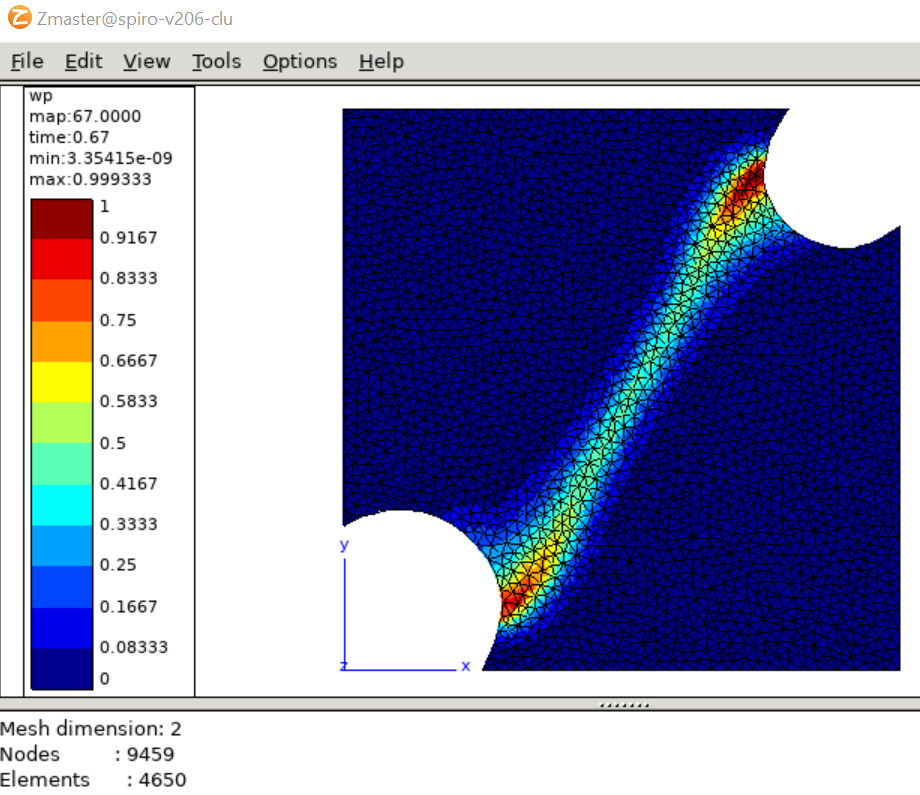
\includegraphics[height=.5\textheight]{calcul_zset.PNG}
\caption{Champ d'endommagement (dénoté $\omega _p$) obtenu avec Zset au temps 0.67s.}
\label{fig:zset}
\end{figure}

\begin{questions}
\question Où vous attendez-vous à voir une fissure? Vous pouvez utiliser les fonction d'Adobe pour l'indiquer sur le pdf afin de pouvoir comparer le résultat final à votre prédiction ou utiliser les outils de graphisme sur une capture d'écran.?
\end{questions}

L'analyse de ce champ 2D se fera à l'aide d'un script en Python. Pour démarrer, ouvrir le fichier \texttt{TP9\_a\_completer.py}.

\section{Charger les données}
A l'aide d'un script de post-processing, les valeurs du champs d'endommagement et du champ de plasticité cumulée non locale à partir duquel ce dernier a été calculé ont été stockés dans le fichier \texttt{calcul.post}. Ce fichier se présente sous la forme suivante: 
\begin{lstlisting}
# ===  time  1.0000000000e-02
#  elem  ip  X  Y  epcum_bar_max  wpmax  
1  1  2.0374861000e+00  8.0624543167e+00  0.0000000000e+00  0.0000000000e+00  
1  2  2.0541407500e+00  7.9675034167e+00  0.0000000000e+00  0.0000000000e+00  
1  3  2.1614351500e+00  8.0264306667e+00  0.0000000000e+00  0.0000000000e+00  
#  elem  ip  X  Y  epcum_bar_max  wpmax  
2  1  1.2305356833e+00  2.8549687500e+00  0.0000000000e+00  0.0000000000e+00  
2  2  1.3302389833e+00  2.8376767000e+00  0.0000000000e+00  0.0000000000e+00  
2  3  1.2638439333e+00  2.9345601500e+00  0.0000000000e+00  0.0000000000e+00  
#  elem  ip  X  Y  epcum_bar_max  wpmax  
[...]
\end{lstlisting}
Dans ce fichier, \texttt{wpmax} désigne l'endommagement et \texttt{epcum\_bar\_max} désigne la plasticité cumulée non locale. Pour chaque élément \texttt{elem}, il y a trois points d'intégration pour lesquels les positions suivant les axes \texttt{X} et \texttt{Y} sont spécifiées. S'agissant d'un calcul mené avec le formalisme des petites déformations, ce sont les positions dans la configuration de référence qui sont précisées. Notons qu'il n'est donc utile de charger les positions des points d'intégration qu'une seule fois.\\

\begin{questions}
\question A partir de l'exemple fourni pour le temps 0.50s, charger les données pour le temps 0.67s et vérifier à l'aide du graphique que la carte obtenue correspond bien à ce qui est présenté en figure~\ref{fig:zset}.
\end{questions}

\section{Distinguer les différentes zones d'amorçage possibles}
Pour ce calcul, deux fissures peuvent apparaître: une au niveau de chaque encoche. Il est plus simple de traiter chaque fissure indépendamment tant qu'elles ne sont pas près de se rencontrer. En effet, un traitement générique peut alors être appliqué à chaque fissure en ne considérant que les points fortement endommagés qui l'entourent. 

\begin{questions}
\question En enlevant le mode commentaire pour le bloc """Select only the higly damaged areas""", tester différentes valeurs de seuil pour déterminer celles qui vous permettent d'obtenir deux groupes distincts de points dont l'endommagement dépasse ce seuil. Attention à faire en sorte d'avoir suffisamment de points dans chaque groupe pour pouvoir exploiter les données. Pour la suite, il est recommandé de prendre la valeur threshold\_damage~=~0.6.
\begin{solution}
Si la valeur de seuil est trop basse, il n'y a qu'un seul groupe. Si la valeur est trop élevée, il n'y aura pas assez de données dans chaque groupe.
\end{solution}
\uplevel{Pour le moment, cette distinction en deux groupes n'est que visuelle. Il reste encore à la programmer pour obtenir deux listes de points distinctes. Au sein d'un code de calcul par éléments finis, il est possible d'utiliser la connectivité des éléments via les n\oe uds pour déterminer des ensembles de points endommagés voisins. Ne disposant pas de cette notion ici, il est possible de faire appel à une fonction de regroupement disponible dans la librairie Python \texttt{sklearn.cluster}: DBSCAN (Density-Based Spatial Clustering of Applications with Noise). Cette fonction va attribuer un \texttt{label} à chaque groupe sous forme d'entier à partir de 0 (-1 étant réservé aux points n'appartenant pas à un groupe particulier et pouvant donc être considéré comme du bruit). Pour l'utiliser, il faut enlever le mode commentaire pour le bloc '''Use DBSCAN to separate the damaged areas'''.\\}

\question En considérant les valeurs dans \texttt{labels}, combien de groupes avez-vous ?
\begin{solution}
Il faut obtenir deux groupes distincts. Il ne devrait pas y avoir de bruit, donc que deux labels: 0 et 1.
\end{solution}

\uplevel{A partir de maintenant, chacune des deux zones sera considérée indépendamment et toutes les analyses suivantes seront effectuées dans une boucle abordant une zone à la fois.}
\end{questions} 

\section{Sélectionner les informations utiles dans chaque zone}
Afin de traiter plus facilement chaque groupe de points, il est utile de définir des listes propres à chaque zone de positions de points d'intégration et de valeur d'endommagement (\texttt{local\_X\_position, local\_Y\_position} et \texttt{local\_damage}).\\

\begin{questions}
\question En vous aidant de \texttt{labels}, compléter le bloc '''Consider each damaged area independently''' pour remplir les listes de données propres à chaque zone ci-dessus.

\begin{solution}
\begin{lstlisting}
for i in indices[0]:
    local_X_position.append(X_position_with_high_damage[i])
    local_Y_position.append(Y_position_with_high_damage[i])
    local_damage.append(high_damage[i])
\end{lstlisting}  
\end{solution} 
\end{questions}

\section{Où insérer le premier incrément de fissure?}

La prochaine étape consiste ensuite à trouver le support du premier incrément de fissure.
\begin{questions}

\uplevel{\subsection{Détermination d'un premier point sur la fissure}\label{sec:premier_point}
La plupart des méthodes commencent par déterminer un premier point censé appartenir à la future fissure. Le plus simple, en dimension 2, est de choisir le point avec le maximum d'endommagement dans la zone.}

\question Dans le bloc '''Find the point with maximum damage''', sélectionner le point avec l'endommagement maximal dans la zone et stocker ses coordonnées dans $(\texttt{X\_max\_damage, Y\_max\_damage})$. Vérifiez visuellement sa position sur la carte d'endommagement.

\begin{solution} Il faut utiliser la fonction \texttt{argmax} de numpy.
\begin{lstlisting}
index_max = np.argmax(local_damage)
X_max_damage = local_X_position[index_max]
Y_max_damage = local_Y_position[index_max]

plt.scatter(local_X_position, local_Y_position, c=local_damage, cmap="jet")
plt.colorbar(orientation="vertical")
plt.title("Maximum damage point marked with a star for area with label %d"%(label))
plt.scatter(X_max_damage, Y_max_damage, color = "black", marker="*", s=100, label='maximum damage')
plt.axis("equal")
plt.legend()
plt.show()  
\end{lstlisting}
Notez que la position du point avec le maximum d'endommagement ne se situe pas sur le bord, là où elle serait attendue. Cela est dû à l'utilisation d'une méthode de régularisation pour calculer le champ étudié, ici la méthode non locale avec gradient implicite. Vu le faible écart, ce n'est pas un problème tant que le premier incrément de fissure intersecte également le bord de l'éprouvette.
\end{solution}


\uplevel{\subsection{Détermination d'un autre point sur la fissure}\label{sec:autre_point}

\paragraph{Positionnement de points d'échantillonnage\\}
Pour déterminer un premier incrément (ou segment en 2D) de fissure, il faut un autre point sur la fissure. Il faut donc chercher un autre point où l'endommagement est maximal. Différentes possibilités existent. Si le point d'endommagement maximal se situe sur un bord, alors il suffit de chercher \emph{le} prochain point où l'endommagement est maximal à une certaine distance (via un calcul de barycentre de points suffisamment endommagés ou la recherche du maximum de la projection de l'endommagement sur une droite). Or, dans le cas présent, le premier point n'est pas sur un bord mais à l'intérieur du domaine. Il faut donc déterminer non pas une, mais deux direction de fissuration possibles. Nous allons donc utiliser le même principe que celui du Marching Ridges afin de déterminer plusieurs directions simultanément: évaluer dans un repère cylindrique les angles correspondant à des maxima relatifs d'endommagement.}

\question En enlevant le mode commentaire pour la partie '''Position evaluation points on a circle''', faire varier la valeur du rayon où sont positionnés les points d'évaluation autour de la valeur recommandée. Pourquoi faut-il éviter de choisir un rayon beaucoup plus grand? Quels sont les inconvénients à choisir un rayon beaucoup plus petit?
\begin{solution}
La valeur proposée (0.15), permet d'aller le plus loin possible tout gardant le cercle dans la zone de points sélectionnée pour une valeur seuil d'endommagement de 0.6. Au-delà, on va manquer d'informations pour évaluer l'endommagement. On risque également d'approcher un chemin de fissure un peu courbe par une droite: il faut faire attention à prendre un rayon suffisamment petit pour capturer la courbure locale. Il ne faut cependant pas choisir un rayon trop petit pour éviter de rester dans une zone de très fort endommagement où on ne pourra pas facilement distinguer la crête.
\end{solution}

\paragraph{Évaluation de l'endommagement aux points d'échantillonnage\\}\label{par:evaluation_damage}

\uplevel{L'objectif des points d'échantillonnage est de permettre une analyse de l'évolution de l'endommagement. Afin d'évaluer l'endommagement, la fonction \texttt{second\_order\_ polynomial\_approximation} a été définie pour fournir une approximation par moindres carrés de la valeur de l'endommagement à un point donné. Cette fonction se sert de la valeur de l'endommagement aux 13 points les plus proches pour estimer au mieux les coefficients d'un polynôme de second ordre.}

\question Reprendre la valeur proposée du rayon (0.15) et enlever le mode commentaire du bloc '''Evaluate damage on the circle'''. Visualiser pour un point d'échantillonnage donné les points les plus proches utilisés pour évaluer la valeur et imprimer les valeurs d'endommagement correspondantes ainsi que la valeur approchée au point d'échantillonnage. Cette dernière vous semble-t-elle correcte?

\begin{solution}
\begin{lstlisting}
if eval_point == 0:
    print("damage_sample", damage_sample)
    print("estimated_damage", estimated_damage)
    plt.scatter(local_X_position, local_Y_position, c=local_damage, cmap="jet")
    plt.colorbar(orientation="vertical")
    plt.scatter(
        X_max_damage,
        Y_max_damage,
        color="black",
        marker="*",
        s=100,
        label="maximum damage",
    )
    plt.scatter(
        X_evaluation_point_position[eval_point],
        Y_evaluation_point_position[eval_point],
        color="gray", 
        marker="x",
        s=50,
        label="evaluation point",
    )
    plt.scatter(X_sample, Y_sample, color="blue", marker="x", s=50, label="sampling points")
    plt.axis("equal")
    plt.legend()
    plt.title("Sampling points are used to estimate damage at each evaluation point")
    plt.show()
\end{lstlisting}
\end{solution}
\question Vérifier visuellement les valeurs d'endommagement obtenues pour tous les points d'évaluation par rapport aux valeurs des points avoisinants. Ces valeurs vous semblent-t-elles correctes?

\question Tracer l'évolution de l'endommagement en fonction de l'angle. Selon vous, quelles sont les directions correspondant à la crête d'endommagement?

\begin{solution}
\begin{lstlisting}
plt.plot(evaluation_angles, approx_damage, "*-", color="blue")
plt.title(
    "Evolution of damage with the angular position between %d" % evaluation_angles[0]
    + " and %d degrees" % evaluation_angles[-1]
)
plt.show()
\end{lstlisting}
Les tendances globales montrent deux directions correspondant à la crête. Cependant, on peut déjà remarquer que le signal est bruité et qu'il y a plus de maxima locaux que voulu.
\end{solution}

\paragraph{Évaluation de l'endommagement aux points d'échantillonnage\\}

\question Enlever le mode commentaire sur le bloc """Damage evolution analysis to find relative max values""" pour trouver les valeurs relatives maximales données par la fonction \texttt{argrelmax} de \texttt{scipy.signal}. Est-ce que cela correspond à vos attentes? Pourquoi avoir pris la peine de définir le nouvel array \texttt{wrappped\_approx\_damage}?\\

\begin{solution}
Avec les valeurs estimées, on se retrouve avec des maxima locaux non désirés dûs au fait que la courbe n'est pas suffisamment lisse. L'array \texttt{wrappped\_approx\_damage} sert à prendre en compte le cas où il y aurait un maximum relatif pour la direction zéro degrés.\end{solution}


\uplevel{\paragraph{Réduire la dépendance à la discrétisation\\}

Avec les données brutes, il peut y avoir trop de bruit pour trouver les 2 directions attendues pour chaque zone. On voit ici l'influence de la discrétisation du calcul par éléments finis qui explique que le recours à un pré-traitement de lissage des données avant analyse par les algorithmes de \emph{crack path tracking}. D'une manière générale, la solution consiste à lisser le champ scalaire étudié en entrée et à utiliser des moyennes sur plusieurs rayons pour déterminer les directions. Pour ce TP, une solution plus économique est simplement de lisser la courbe, par exemple à l'aide d'un filtre de Savitzky-Golay.}

\question Enlever le mode commentaire sur le bloc """Damage evolution analysis on smoothed curved to find relative max values""" pour trouver les valeurs relatives maximales données par la fonction \texttt{argrelmax} de \texttt{scipy.signal}. Est-ce que cela correspond plus à vos attentes?

\question Tracer les segments correspondants pour chaque zone et vérifier la cohérence par rapport aux points endommagés sélectionnés.

\begin{solution}
\begin{lstlisting}
for num_branch in np.arange(0, len(max_indices)):
    X_ridge_point = X_max_damage + radius * math.cos(
        wrapped_evaluation_angles[max_indices[num_branch]] * math.pi / 180.0
    )
    Y_ridge_point = Y_max_damage + radius * math.sin(
        wrapped_evaluation_angles[max_indices[num_branch]] * math.pi / 180.0
    )      
\end{lstlisting}
\end{solution}
\end{questions}


\section{Jusqu'où insérer le premier incrément de fissure?}

Une fois le support d'une fissure déterminé, il reste à savoir quelle partie de ce support correspond réellement à un incrément de fissure à insérer. On fait pour cela appel à un critère d'insertion qui compare la valeur de l'endommagement à une valeur critique. 

\begin{questions}
\uplevel{\subsection{Évaluer l'endommagement le long du support}
}
\question Pour chaque direction de fissure possible, distribuer des points pour y évaluer l'endommagement. Vous pouvez choisir de distribuer une vingtaine de points avec un pas égal à 20\% du rayon considéré. Stocker leurs coordonnées dans les listes \texttt{X\_on\_segment} et \texttt{Y\_on\_segment} et les valeurs d'endommagement correspondantes dans une liste nommée \texttt{damage\_on\_segment}.

\begin{solution}
\begin{lstlisting}
for multip in np.arange(0, 20):
    new_radius = multip * delta_L
    X_point = X_max_damage + new_radius * math.cos(
        wrapped_evaluation_angles[index_angle] * math.pi / 180.0
    )
    Y_point = Y_max_damage + new_radius * math.sin(
        wrapped_evaluation_angles[index_angle] * math.pi / 180.0
    )
    X_sample, Y_sample, damage_sample = find_closest_points(
        X_point, Y_point, local_X_position, local_Y_position, sample_size, local_damage
    )
    estimated_damage = second_order_polynomial_approximation(
        X_point, Y_point, X_sample, Y_sample, damage_sample
    )
    X_on_segment.append(X_point)
    Y_on_segment.append(Y_point)
    damage_on_segment.append(estimated_damage)
\end{lstlisting}
\end{solution}

\uplevel{\subsection{Utiliser un critère d'insertion}\label{sec:critere_insert}

Il faut enfin choisir une valeur d'endommagement suffisamment proche de la borne supérieure (1) qui corresponde à l'apparition d'une fissure: considérons par exemple 0.95.}

\question Tracer l'évolution de l'endommagement en fonction des coordonnées suivant l'axe X des points d'échantillonnage et ainsi que la droite correspondant à la valeur limite dans une même figure pour chacun des supports de fissure envisagé.
\begin{solution}
\begin{lstlisting}
plt.plot(X_on_segment, damage_on_segment, color="black", label="damage")
plt.plot(
    X_on_segment,
    limit_damage * np.ones(len(X_on_segment)),
    color="red",
    label="limit value of %f" % limit_damage,
)
plt.title(
    "Evolution of damage along the X-axis for angle: %d deg"
    % wrapped_evaluation_angles[index_angle]
)
plt.legend()
plt.show()
\end{lstlisting}
\end{solution}
\question Combien de segments de fissure sont à insérer?

\begin{solution}
Pour la première zone, en bas à gauche, les valeurs d'endommagement sont en-dessous du seuil. Pour la seconde zone, en haut à droite, une partie de chacun des deux segments correspond à un endommagement suffisamment élevé pour être insérée.
\end{solution}

\question En comparant la valeur d'endommagement à chacun des points d'échantillonnage à la valeur critique, ne sélectionner que les points sur la partie du support à insérer et stocker leurs coordonnées dans les listes \texttt{selected\_X\_on\_segment} et \texttt{selected\_Y\_on\_segment}. Une précision de l'ordre de 20\% du rayon d'évaluation sera suffisante ici pour comprendre les grands principes.

\begin{solution}
\begin{lstlisting}
for index_point in np.arange(0,len(X_on_segment)):
            estimated_damage = damage_on_segment[index_point]
            if estimated_damage >= limit_damage:
                selected_X_on_segment.append(X_on_segment[index_point])
                selected_Y_on_segment.append(Y_on_segment[index_point])
                
\end{lstlisting}
\end{solution}

\question Tracer les parties à insérer pour chaque support.
\begin{solution}
\begin{lstlisting}
plt.scatter(local_X_position, local_Y_position, c=local_damage, cmap="jet")
plt.colorbar(orientation="vertical")
plt.scatter(
    X_max_damage, Y_max_damage, color="black", marker="*", s=100, label="maximum damage"
)
plt.plot(selected_X_on_segment, selected_Y_on_segment, "-*", c="black")
plt.axis("equal")
plt.legend()
plt.title(
    "Part of the segments above limit damage for angle: %d deg"
    % wrapped_evaluation_angles[index_angle]
)
plt.show()
\end{lstlisting}
\end{solution}

\question Stocker les coordonnées des points extrémités des segments dans les listes \texttt{X\_all\_segments} et \texttt{Y\_all\_segments} définies au début du fichier. Tracer les parties à insérer pour chaque support.

\begin{solution}
\begin{lstlisting}
if len(selected_X_on_segment) > 0:
    X_all_segments.append([X_max_damage, selected_X_on_segment[-1]])
    Y_all_segments.append([Y_max_damage, selected_Y_on_segment[-1]])
\end{lstlisting}
\end{solution}
\end{questions}

\section{Résultat final}
\begin{questions}
\question En vous aidant des listes \texttt{X\_all\_segments} et \texttt{Y\_all\_segments}, tracer tous les segments de fissure à insérer sur la carte d'endommagement initiale pour la comparer qualitativement avec votre prédiction.
\begin{solution}
\begin{lstlisting}
plt.scatter(X_position, Y_position, c=damage, cmap="jet", marker=".")
plt.colorbar(orientation="vertical")
for index in np.arange(0, len(X_all_segments)):
    plt.plot(X_all_segments[index], Y_all_segments[index], "-*", c="black")
plt.axis("equal")
plt.title("Crack increments ready for insertion for time %f" % selected_time)
plt.show()
\end{lstlisting}
\end{solution}
\end{questions}

\section{Pour aller plus loin}
La combinaison de choix qui vous ont été proposés a permis d'obtenir une discrétisation de la fissure (ou des fissures) à insérer dans le modèle. Comme illustré dans le cours, d'autres options sont possibles pour chaque étape. Si vous en avez le temps, voici quelques options à explorer:
\begin{itemize}
\item Reprendre la recherche d'un premier point sur la fissure~(\ref{sec:premier_point}) en cherchant le barycentre de points suffisamment endommagés. 
\item Reprendre la détermination d'un autre point sur la fissure~(\ref{sec:autre_point}) en utilisant une régression linéaire sur la position des points les plus endommagés pour approcher le premier incrément de fissure par un segment de droite. 
\end{itemize} 
De la même manière, le code obtenu permet de traiter un cas particulier de manière satisfaisante. Pour traiter plus de cas de manière plus robuste, des petites modifications sont possibles et peuvent être également explorées:
\begin{itemize}
\item utiliser le champ (non borné) de plasticité cumulée non locale pour la direction et le champ d'endommagement pour le critère d'insertion;
\item ajouter une fonction poids dans l'approximation par moindres carrés (\ref{par:evaluation_damage}) pour donner moins de poids aux points d'échantillonnage les plus éloignés;
\item déterminer plus précisément la position de la pointe de fissure pour~\ref{sec:critere_insert} grâce à une interpolation linéaire en se servant des coordonnées et des valeurs aux points avant et après intersection avec la valeur critique.
\end{itemize}
Enfin, seule l'étape d'amorçage a été traitée. Il est possible d'aller plus loin en:
\begin{itemize}
\item programmant la recherche du prochain point sur la crête à partir des extrémités pertinentes pour la même carte (\emph{exhaustion method});
\item programmant la recherche pour tous les pas de temps en exploitant les segments déjà trouvés (propagation de fissure).
\end{itemize}
N'hésitez pas à tester les pistes qui vous inspirent!


\end{document}